\documentclass[12pt]{book}
\usepackage{standalone}
\usepackage{apacite}
\usepackage{etoolbox}% for the \patchcmd
\makeatletter
% Patch after apacite got loaded!
\patchcmd{\nocite}{\@onlypreamble\document}{\documentclass\sa@documentclass}{}{}
\makeatother
\usepackage{graphicx}
\usepackage{subcaption}
\graphicspath{{C:/Users/huawei/Desktop/images/}} 
\usepackage{setspace}
\usepackage{booktabs}
\usepackage{tabularx}
\usepackage{xcolor}
\usepackage{amsmath}
\usepackage{pdflscape}
\usepackage[margin=3cm]{geometry}
\usepackage{multirow}
\usepackage{times}
\usepackage{fancyhdr}
\usepackage{color}
\usepackage{dcolumn}
\usepackage{siunitx}
\usepackage{array}
\usepackage{longtable}
%\usepackage{forest}
\usepackage{tikz}
\usetikzlibrary{shapes.geometric, arrows}
\tikzstyle{startstop} = [rectangle, minimum width=1.5cm, minimum height=1cm,text centered, draw=black]
\tikzstyle{process} = [rectangle, rounded corners, minimum width=0.5cm, minimum height=1cm, text width =2.5cm, text centered, draw=black]
\tikzstyle{arrow} = [thick,->,>=stealth]

\raggedbottom

\renewcommand\baselinestretch{2}


\newcolumntype{d}[1]{D{.}{.}{#1}}
\def\sym#1{\ifmmode^{#1}\else\(^{#1}\)\fi}


\begin{document}
\chapter{Formal modeling}\label{chap:formalModel}

This chapter provides a brief overview of the formal models introduced for modeling IAT data. 
These models are generally aimed at the investigation of the cognitive processes and the automatic associations involved during the performance at the IAT. Their advantages and drawbacks are outlined and discussed.

Some of these models  are solely based on accuracy responses (Section \ref{sec:multimodel}), while others are able to concurrently model accuracy and time responses (Section \ref{sec:timeacc}).
Despite the important and useful information provided at the sample level and/or the stimuli categories level, none of these models provides detailed information at the singular stimulus level.

The Rasch modeling of IAT data can overcome this issue, as illustrated in Section \ref{sec:mfrm}. Although this approach provides stimulus-specific information, it also comes with some drawbacks, mostly related to the discretization of response times and to the overlooking of the fully-crossed structure of the IAT.


\section{Multinomial Models}\label{sec:multimodel}
\subsection{The Quad Model}\label{sub:quad}
The Quad model \cite{Conrey2005} is a multinomial processing tree model introduced for distinguishing the contribution of automatic processes from that of controlled processes in driving respondents' performances at the IAT. 
The Quad model is entirely based on accuracy responses, and it exploits the logic of the assumption on which the IAT is based (i.e., response compatibility, according to which responses are faster and more accurate in the condition consistent with one's automatically activated associations). 

According to this model, the observed accuracy responses are determined by the activation (or lack of thereof) of four qualitatively different processes, characterized by different levels of automaticity and controllability.
These processes are the automatic activation of an association triggered by the target stimulus (\emph{activation association}, AC), the ability to correctly identify the category to which the stimulus belongs (\emph{discriminability}, D), the ability to overcome any automatically activated associations (\emph{overcoming bias}, OB), and the influence of any response bias that may intervene in absence of any other process (\emph{guessing}, G). A graphical representation of the Quad model is provided in Figure \ref{fig:quad}.

	\begin{landscape}
	\begin{figure}
		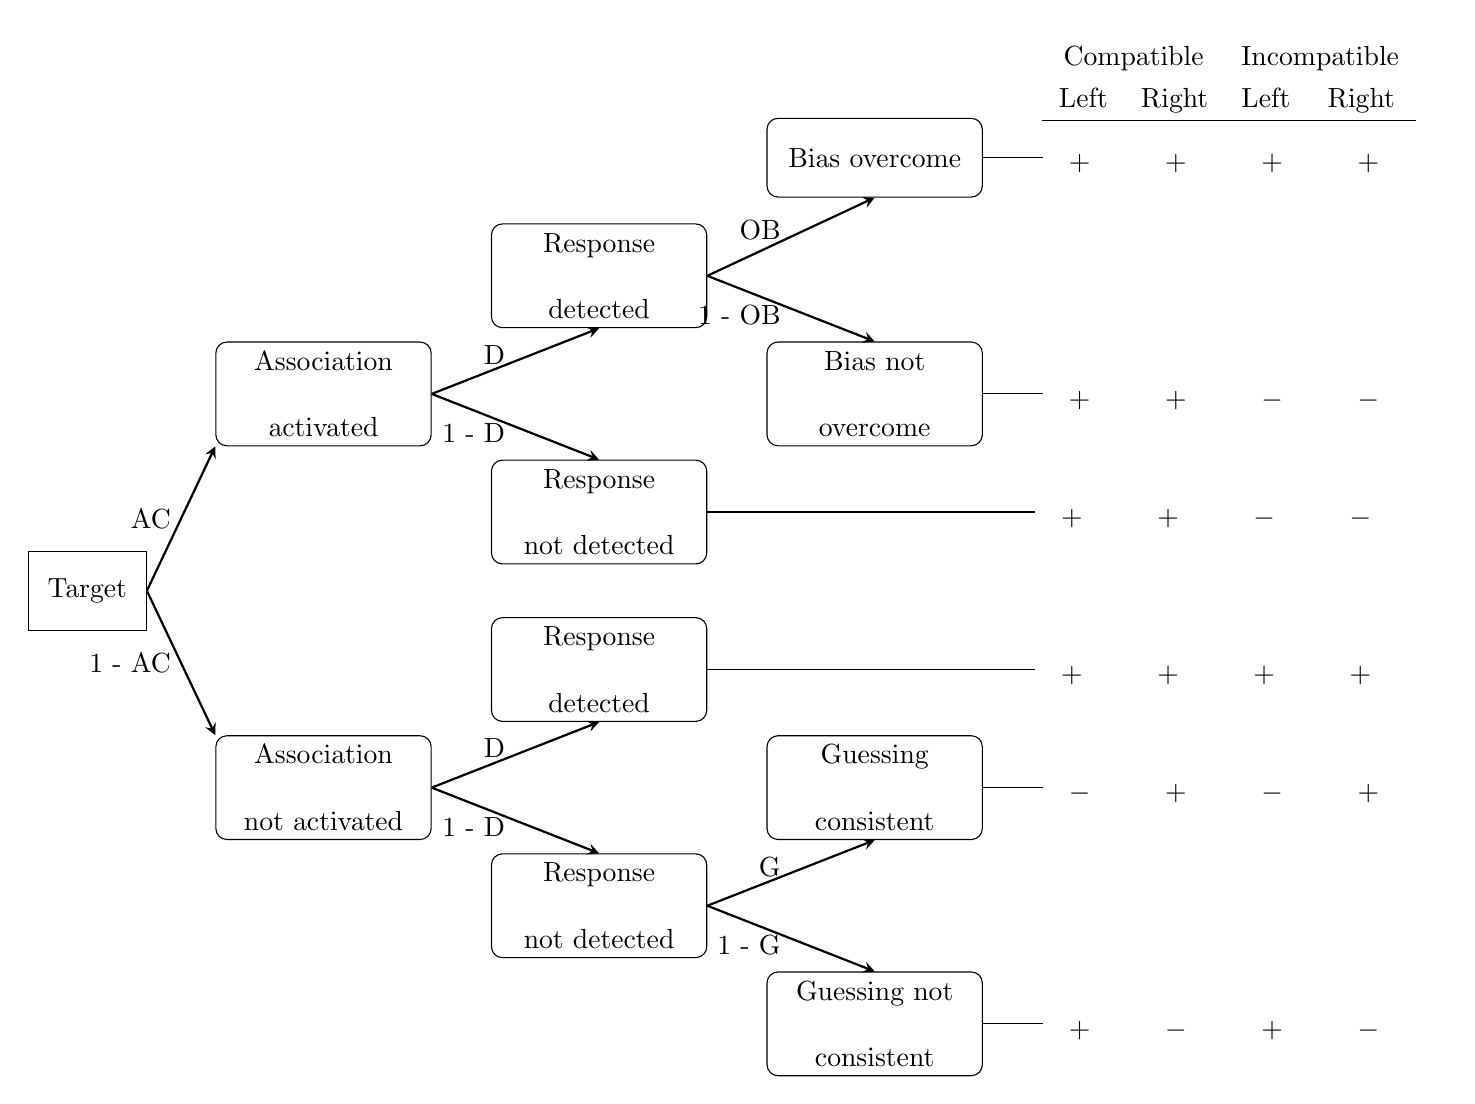
\begin{tikzpicture}[node distance=2cm]
			\node (start) [startstop] {Target};
			\node (ac) [process, right of = start, yshift=2.5cm, xshift = 1cm] {Association activated};
			\node (notac) [process, right of = start, yshift=-2.5cm, xshift = 1cm] {Association not activated};
			\node (d) [process, right of = ac, yshift=1.5cm, xshift = 1.5cm] {Response detected};
			\node (notd) [process, right of = ac, yshift=-1.5cm, xshift = 1.5cm] {Response not detected};
			\node (ob) [process, right of = d, yshift=1.5cm, xshift = 1.5cm] {Bias overcome};
			\node (notob) [process, right of = d, yshift=-1.5cm, xshift = 1.5cm] {Bias not overcome};
			\node (d1) [process, right of = notac, yshift=1.5cm, xshift = 1.5cm] {Response detected};
			\node (notd1) [process, right of = notac, yshift=-1.5cm, xshift = 1.5cm] {Response not detected};
			\node (g) [process, right of = notd1, yshift=1.5cm, xshift = 1.5cm] {Guessing consistent};
			\node (notg) [process, right of = notd1, yshift=-1.5cm, xshift = 1.5cm] {Guessing not consistent};
			\path [arrow] (start.east) edge node[anchor=east] {AC} (ac.south west);
			\path [arrow] (start.east) edge node[anchor=east] {1 - AC} (notac.north west);
			\path [arrow] (ac.east) edge node[anchor=east, yshift = 0.08cm] {D} (d.south);
			\path [arrow] (ac.east) edge node[anchor=east, yshift = -0.08cm] {1 - D} (notd.north);
			\path [arrow] (d.east) edge node[anchor=east, yshift = 0.08cm] {OB} (ob.south);
			\path [arrow] (d.east) edge node[anchor=east, yshift = -0.08cm] {1 - OB} (notob.north);
			\path [arrow] (notac.east) edge node[anchor=east, yshift = 0.08cm] {D} (d1.south);
			\path [arrow] (notac.east) edge node[anchor=east, yshift = -0.08cm] {1 - D} (notd1.north);
			\path [arrow] (notd1.east) edge node[anchor=east, yshift=0.08cm] {G} (g.south);
			\path [arrow] (notd1.east) edge node[anchor=east, yshift = -0.08cm] {1 - G} (notg.north);
			
			\node (table) [rectangle ,right of = ob, xshift = 2.5cm, yshift = 1cm]{%
				\onehalfspacing
				\begin{tabular}{c c c c}
					\multicolumn{2}{c}{Compatible} & \multicolumn{2}{c}{Incompatible}\\
					
					\multicolumn{1}{c}{Left} & \multicolumn{1}{c}{Right} & \multicolumn{1}{c}{Left} & \multicolumn{1}{c}{Right} \\
					\hline
				\end{tabular}
			};
			\node (first) [rectangle ,right of = ob, xshift = 2.7cm] {%
				\begin{tabular}{p{0.8cm} p{0.8cm} p{0.8cm} p{0.8cm}}
					$+$ & $+$ & $+$ & $+$ \\
			\end{tabular}};
			\node (second) [rectangle ,right of = notob, xshift = 2.7cm] {%
				\begin{tabular}{p{0.8cm} p{0.8cm} p{0.8cm} p{0.8cm}}
					$+$ & $+$ & $-$ & $-$ \\
			\end{tabular}};
			\node (third) [rectangle ,right of = notd, xshift = 6.1cm] {%
				\begin{tabular}{p{0.8cm} p{0.8cm} p{0.8cm} p{0.8cm}}
					$+$ & $+$ & $-$ & $-$ \\
			\end{tabular}};
			\node (fourth) [rectangle ,right of = d1, xshift = 6.1cm] {%
				\begin{tabular}{p{0.8cm} p{0.8cm} p{0.8cm} p{0.8cm}}
					$+$ & $+$ & $+$ & $+$ \\
			\end{tabular}};
			\node (fifth) [rectangle ,right of = g, xshift = 2.7cm] {%
				\begin{tabular}{p{0.8cm} p{0.8cm} p{0.8cm} p{0.8cm}}
					$-$ & $+$ & $-$ & $+$ \\
			\end{tabular}};
			\node (sixth) [rectangle ,right of = notg, xshift = 2.7cm] {%
				\begin{tabular}{p{0.8cm} p{0.8cm} p{0.8cm} p{0.8cm}}
					$+$ & $-$ & $+$ & $-$ \\
			\end{tabular}};
		\path [-] (ob.east) edge (first.west);
		\path [-] (notob.east) edge (second.west);
		\path [-] (notd.east) edge (third.west);
		\path [-] (d1.east) edge (fourth.west);
		\path [-] (g.east) edge (fifth.west);
		\path [-] (notg.east) edge (sixth.west);
		\end{tikzpicture}
		\caption{\label{fig:quad} Quad Model \protect\cite<adapted from>{Conrey2005}. Parameters with arrows pointing towards them are conditional on all the preceding ones. $+$: correct response (stimulus correctly assigned to its category), $-$: incorrect response (stimulus assigned to the incorrect category).}
	\end{figure}
\end{landscape}


  
%Specifically, Quad model is aimed at highlighting the contribution of four qualitatively different processes defined by different levels of automaticity and/or controllability.  It is completely based on accuracy responses, and it exploits the logic of response compatibility. Response compatibility is the assumption on which the IAT rests, namely, that responses are more accurate and faster in the condition compatible with respondent's automatic association. 
%The activation, or lack of thereof, of the four processes contributes to the overt %response in the IAT. 
%The observed probability of a correct response to a particular category of stimuli is the starting point for estimating the four parameters. The sum of the probabilities associated with a response is the total probability of that response. 

Each path in Figure \ref{fig:quad} represents the likelihood that a parameter is activated. The activation of the parameters are conditional on the activation of the parameters preceding them. 

%These processes are represented by four parameters, which are estimated from the observed probability of a correct responses to a specific category of stimuli.
The parameter AC describes the probability that an automatic association is activated by the triggering stimulus. This parameter expresses the most automatic component of the model and it is directly related to the strength of the association activated by the stimulus. The stronger the association between the stimulus and a negative/positive attribute, the more likely the activation of the automatic association.

The probability of giving the correct response does not solely depend on the activation of the automatic association, but also on the ability to identify the correct response among the available responses. This ability in turn depends on the availability of cognitive resources and on the application of some effort in determining the correct response. As such, parameter D represents the likelihood that the correct response \emph{can} be identified, not the likelihood that the correct response \emph{is} identified. The parameter D depends on several factors, including the motivation to have a good performance, the attention paid to the stimulus, and the availability of relevant information in memory.

If a negative automatic association is activated by the triggering stimulus, the respondent might try to fake the response in a socially desirable way. The parameter OB represents the likelihood that an activated bias is overcome in favor of a deliberate, and probably more desirable, response. 

The processes described by the parameters D and OB are the ones that are mostly influenced by motivation and that mostly depend on the availability of cognitive resources  to be activated and to drive the correct response. They do reflect two different aspects of controlled processes. The controlled process involved by the parameter D is an active search for the correct response, while the process described by the parameter OB  exploits control for the inhibition of the response activated by the automatic association. 

If none of the above-mentioned processes is activated, then the responses can be influenced by a response bias, such as the tendency to respond with the left response key. The parameter G represents the likelihood that a response bias, different than the automatic association, is activated and drives the responses. 

As previously mentioned, the parameters of the Quad model are estimated from the observed proportions of a correct response given a stimulus type. Each arrow moving from left to right in Figure \ref{fig:quad} represents the multiplication between the independent probabilities of each process. It results in the prediction of a specific response, either correct or incorrect. 
The sum of all probabilities associated to that response is the total probability of that response.

Consider a respondent with an implicit preference for Pepsi over Coke. For him/her, the incompatible condition is the Coke/Good-Pepsi/Bad condition. The probability that this respondent has of correctly sorting a can of Coke in the incompatible condition is given by the sum of the paths resulting in a correct response. In this case, three processes lead to the correct response. As such, the resulting equation is: $\text{P(correct}|\text{Coke, incompatible)} = AC \times D \times OB + (1-AC)\times D + (1-AC)\times (1-D) \times (1-G)$. 
The first path ($AC \times D \times OB$) represents the probability that an automatic association is activated by the stimulus ($AC$), that the response can be identified ($D$), and that the bias is successfully overcome ($OB$).
The second path  ($(1-AC)\times D$) represents the probability that the automatic association is not activated ($1 - AC$) and that the response can be identified ($D$). 
Finally, the third path ($(1-AC)\times (1-D) \times (1-G)$) represents the probability that the association is not activated ($1-AC$), the correct response cannot be detected ($1-D$), and that automatically responding with the left response key is not an effect of guessing ($1-G$).
The sum of the products of the independent probabilities yielded by each path results in the total probability of a correct response to the stimulus.


By qualitatively disentangling the nature of the processes intervening during the performance at the IAT, the Quad model offers detailed information on the IAT functioning. 
Most importantly, the Quad model explicitly points out that the performance at the IAT should not be taken as the sole expression of automatic processes. Rather, the contribution of controlled processes should be acknowledged and taken into account for the explanation of social phenomena. 

This point has crucial repercussion on applied researches using the IAT.
For instance, in an IAT for the assessment of implicit prejudice, it would be of the uttermost importance to understand whether a resulting negative \emph{D} score (e.g., a \emph{D} score indicating preference for White people over Black people) is actually due to the automatic activation of the association between one of the targeted groups and negative attributes or to other, more controlled, processes, such as the inability to identify the correct response.  
The information provided by the OB parameter allows for understanding whether a positive \emph{D} score is the expression of genuinely automatic associations between the stigmatized group and positive attributes or by the desire to conceal negative attitudes towards the stigmatized group.
Both the parameters AC and OB are associated with the typical IAT \emph{D} score \cite{Conrey2005}.
The \emph{D} score was found to be positively associated with the parameter AC (i.e., the stronger the association activated by the stimulus, the higher the \emph{D} score value). 
Moreover, the parameter AC allowed for pinpointing the contribution of distinct associations in a Race IAT, according to which both White-pleasant  automatic associations and Black-unpleasant ones were related with the \emph{D} score. The \emph{D} score is hence capturing two distinct associations, and it is confounding them into a unique score. 
%It ca be speculated that the IAT effect as expressed by the \emph{D} score does measure two distinct associations. 
%Grounding on this evidence, the typical IAT \emph{D} score is not able to disentangle the controlled processes from the automatic ones. As such, it cannot be used as a measure of automatic bias.
%AC parameter has been found to vary according to associations, not stimulus type, also in a Flowers-Insects IAT.
The \emph{D} score was negatively associated to the ability of suppressing an automatic activated association described by the parameter OB. The higher the ability to overcome the bias, and hence the value of OB, the lower the IAT effect as expressed by the \emph{D} score.
%OB parameter, that is the likelihood of successfully overcoming an automatic bias, was negatively associated with the \emph{D} score. In other words, the higher the probability of giving the correct response despite an automatic association has been activated the lower the value of the \emph{D} score. 

Grounding on these evidence, it can be said that the \emph{D} score confounds different information into a single, generic score. Firstly, it is not possible to ascertain which of the specific automatic associations drives the performance at the IAT, leaving its meaning partially obscure. 
Moreover, controlled and automatic processes cannot be distinguished from one another, and their unique contribution is lost. It is not possible to ascertain whether the performance is driven by an actual automatic association or if the IAT effect reflects the respondents' ability to detect the correct response or their ability of overcoming an automatic activated bias. 
It appears evident that distinguishing between these processes is extremely important when inferences on sensitive psychological constructs, such as implicit bias, are made. Indeed, the implications of saying that a sample of individuals is implicitly biased towards a social group are extremely different from saying that the sample has a high ability in detecting the correct responses.
The \emph{D} score alone cannot be used as a measure of pure implicit bias.

The information provided by the Quad model are extremely useful and meaningful for a correct interpretation of the IAT effect. 
However, it should be taken with caution for at least two reasons: The results are entirely based on accuracy responses and the persons' estimates are at the sample level and not at the individual respondent's level.

Regarding the first issue, the IAT is known to be an easy task -- it is actually designed to be an easy task by choosing highly representative and easily sortable stimuli. As such, the error rates are extremely low, unless the respondent was distracted or the task itself did not work properly. This raises issues concerning the estimation of the model parameters and their reliability. Moreover, not using the time responses implies losing the majority of the information that can be retrieved from the IAT data, which can in turn lead to an incorrect interpretation of the results. 
For instance, the higher accuracy of the responses when the automatic associations is activated might be also associated to slower response times \cite<speed-accuracy trade-off,>{Klauer2007}. By considering only the accuracy responses, the Quad model is not able to rule out this possibility, and the conclusions based on the Quad model might be misleading.
%Despite interesting, this result should be taken with caution. Indeed, the Quad model, and the estimation of its parameters, is solely based on the accuracy responses. There are reasons to believe that higher accuracy of the responses when an automatic bias is activated might be associated to slower response times (speed-accuracy trade-off). The Quad model is not able to rule out this possibility, hence the conclusions based on this result might be misleading. 
The parameter OB is the one controlling the accuracy of the responses when an automatic association is activated, and, as such, it should be the one mostly affected by the speed-accuracy trade-off. Indeed, results of Study 2 in \citeA{Conrey2005} actually pointed in this direction. The parameter OB dropped significantly (i.e., respondents with automatically activated associations were not able anymore to provide the correct response) when a time constraint for giving the response was introduced.
This result does indicate that the parameter OB captures a controlled process that needs time to be activated and successfully used. 
Not considering response times for interpreting the results on the parameter OB appears to be a fallacy leading to incorrect or misleading inferences.

Regarding the second issue, the estimates provided by the Quad model are at either the sample level or the stimuli categories level. 
Consequently, both the between--respondents variability and the between--stimuli one are completely ignored. 
Moreover, having sample estimates at the sample level for the respondents does not allow for investigating the respondents' individual differences, which is usually the main objective of applied social psychology. 
Similarly, the information at the level of the singular stimulus is neglected. 

To be fair, in Study 4 in \citeA{Conrey2005} respondent--specific estimates were obtained. 
However, obtaining respondent--specific estimates with the Quad model is tricky given the high error rate needed in the starting contingency table, where stimuli categories are crossed with the associative conditions, within each respondent. To ensure an high error rate value for each possible combination, a longer IAT procedure should be adopted. As such, the Quad model is not feasible for investigating individual differences using IATs of typical length.
%Finally, the estimates provided by the Quad model are either the sample or stimuli category level. Respondent--specific estimates can be obtained as well \cite<e.g., Study 4,>{Conrey2005}, but still the information that can be retrieved from each individual stimulus is not considered.



%According to the Quad Model, the accuracy performance at the IAT depends on four qualitatively distinct processes: (i) the automatic activation of an association triggered by a stimulus, (ii) the ability to discriminate the correct category to which the stimulus belongs, (iii) the ability to overcome automatically activated associations, and (iv) any response bias (e.g., the tendency to respond with the right response key) that may drive the response in absence of any other process. 



\subsection{The ReAL Model}\label{sub:real}

The ReAL model \cite{Meissner2013} is a multinomial processing tree model based on accuracy responses. 
This model is aimed at mathematically distinguishing the contribution of the automatic associations from that of recoding or simplification strategies that might intervene during the performance at the IAT. 

The ReAL model is based on two main assumptions. 
%ReAL model postulates that a part of respondents' performance during the IAT is ascribable to strategies implemented to simplify the categorization task,
The first assumption is that only attitude objects activate automatic evaluative associations. Consequently, evaluative associations influence responding only for attitudes stimuli, while the same does not hold for attributes stimuli. In other words, attitude objects can be sorted according to their evaluative value, while evaluative attributes cannot be sorted according to the attitude objects to which they are associated.
The second assumption logically follows from the first one. To be recoded into a unique category, target stimuli and evaluative attributes must be sharing a common feature, that is, an intrinsic positive or negative value. The common feature shared by the evaluative dimensions and the attitude objects is determined by attitude based associations.
Attitude based associations can facilitate the correct sorting of the target stimuli in the condition consistent with individual's automatically activated association (i.e., compatible) but not in that against individual's own automatically activated association (i.e., incompatible). The recoding of target stimuli according to their evaluative dimension facilitates the performance only in the compatible condition, while it hinders it in the incompatible one.
% Consequently, recoding strategies can positively affect the responding only in the condition where the intrinsic value of the objects and the evaluative attributes are consistent between each other.

For example, in the Coke-Good/Pepsi-Bad condition of a Coke-Pepsi IAT, a respondent with a strong preference for Coke might simplify the task by sorting Coke exemplars according to their positive value. 
As such, the task is reduced from a 4-choice task (i.e., \emph{Coke} and \emph{Good}, \emph{Pepsi} and \emph{Bad}) to a 2-choice task (i.e., \emph{Good}, which also includes \emph{Coke}, and everything else). However, this strategy can work only in the associative condition that is consistent with respondent's automatically activated associations.

Grounding on these assumptions, three processes are assumed to drive the correct and incorrect response pattern in the IAT. Their influence on the performance changes according to the specific IAT associative condition, as illustrated in Figure \ref{fig:real}. The illustration of the ReAL model is based on the Coke-Pepsi IAT example introduced in Chapter \ref{chap:intro}, considering a respondent with a strong preference for Coke over Pepsi.

\begin{landscape}
	\begin{figure}
		\begin{subfigure}{\linewidth}
			\begin{tikzpicture}
				\node[rotate=90, left of = start, yshift=3cm, xshift=1cm] {\large{Compatible condition}};
				\node (start) [startstop] {Target};
				\node (re) [process, right of = start, yshift=1.5cm, xshift = 2cm] {Recoding drives};
				\node (notre) [process, right of = start, yshift=-1.5cm, xshift = 2cm] {Recoding do not drive};
				\node (l) [process, right of = notre, yshift=1.5cm, xshift = 2cm] {Label based};
				\node (notl) [process, right of = notre, yshift=-1.5cm, xshift = 2cm] {Not label based};
				\node (good) [process, right of = notl, yshift=1.5cm, xshift = 2cm] {\emph{Good} automatic associations};
				\node (bad) [process, right of = notl, yshift=-1.5cm, xshift = 2cm] {\emph{Bad} automatic associations};
				\path [arrow] (start.east) edge node[anchor=east, yshift = 0.08cm] {\emph{Re}} (re.south);
				\path [arrow] (start.east) edge node[anchor=east, yshift = -0.08cm] {1-\emph{Re}} (notre.north);
				\path [arrow] (notre.east) edge node[anchor=east, yshift = 0.08cm] {\emph{L}} (l.south);
				\path [arrow] (notre.east) edge node[anchor=east, yshift = -0.08cm] {1-\emph{L}} (notl.north);
				\path [arrow] (notl.east) edge node[anchor=east, yshift = 0.08cm] {\emph{A}} (good.south);
				\path [arrow] (notl.east) edge node[anchor=east, yshift = -0.08cm] {1-\emph{A}} (bad.north);
				
				\node (table) [rectangle ,right of = re, xshift = 10.5cm, yshift = 1.5cm]{%
					\onehalfspacing
					\begin{tabular}{c c}
						\multicolumn{1}{c}{Coke} & \multicolumn{1}{c}{Pepsi}\\
						\hline
					\end{tabular}
				};
				\node (first) [rectangle ,right of = re, xshift = 10.5cm]{%
				\onehalfspacing
				\begin{tabular}{c c}
					$+$ & $+$\\
				\end{tabular}
			};
						\node (second) [rectangle ,right of = l, xshift = 7.5cm]{%
			\onehalfspacing
			\begin{tabular}{c c}
				$+$ & $+$\\
			\end{tabular}
		};
		\node (third) [rectangle ,right of = good, xshift = 4.5cm]{%
			\onehalfspacing
			\begin{tabular}{c c}
				$+$ & $-$\\
			\end{tabular}
		};
			\node (fourth) [rectangle ,right of = bad, xshift = 4.5cm]{%
		\onehalfspacing
		\begin{tabular}{c c}
			$-$ & $+$\\
		\end{tabular}
	};			
\path [-] (re.east) edge (first.west);
\path [-] (l.east) edge (second.west);
\path [-] (good.east) edge (third.west);
\path [-] (bad.east) edge (fourth.west);
			\end{tikzpicture}
			%\caption{\label{subfig:realcomp} Compatible block.}
		\end{subfigure}
		\par\bigskip
		\begin{subfigure}{\linewidth}
			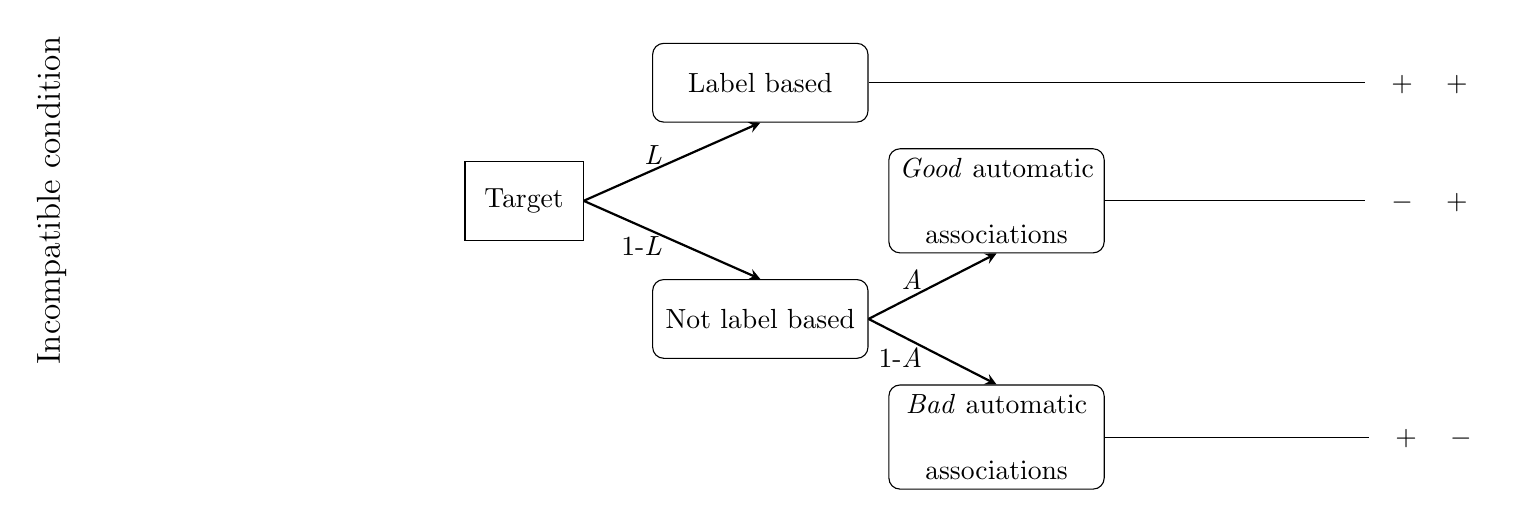
\begin{tikzpicture}
				
				\node (empty) [rectangle] {};
					\node[rotate=90, left of = empty, yshift=3.3cm, xshift=1cm] {\large{Incompatible condition}};
				\node (start) [startstop, right of = empty, xshift = 1.7cm] {Target};
				\node (l) [process, right of = start, yshift=1.5cm, xshift = 2cm] {Label based};
				\node (notl) [process, right of = start, yshift=-1.5cm, xshift = 2cm] {Not label based};
				\node (good) [process, right of = notl, yshift=1.5cm, xshift = 2cm] {\emph{Good} automatic associations};
				\node (bad) [process, right of = notl, yshift=-1.5cm, xshift = 2cm] {\emph{Bad} automatic associations};
				\path [arrow] (start.east) edge node[anchor=east, yshift = 0.08cm] {\emph{L}} (l.south);
				\path [arrow] (start.east) edge node[anchor=east, yshift = -0.08cm] {1-\emph{L}} (notl.north);
				\path [arrow] (notl.east) edge node[anchor=east, yshift = 0.08cm] {\emph{A}} (good.south);
				\path [arrow] (notl.east) edge node[anchor=east, yshift = -0.08cm] {1-\emph{A}} (bad.north);
				
				\node (first) [rectangle ,right of = l, xshift = 7.5cm]{%
					\onehalfspacing
					\begin{tabular}{c c}
						$+$ & $+$\\
					\end{tabular}
				};
				\node (second) [rectangle ,right of = good, xshift = 4.5cm]{%
					\onehalfspacing
					\begin{tabular}{c c}
						$-$ & $+$\\
					\end{tabular}
				};
				\node (third) [rectangle ,right of = bad, xshift = 4.55cm]{%
					\onehalfspacing
					\begin{tabular}{c c}
							$+$ & $-$\\
					\end{tabular}
				};	
			\path [-] (l.east) edge (first.west);
			\path [-] (good.east) edge (second.west);
			\path [-] (bad.east) edge (third.west);	
			\end{tikzpicture}
			%\caption{\label{subfig:realinc}Incompatible Block}
		\end{subfigure}
		\caption{\label{fig:real} ReAL model \protect\cite<adapted from>{Meissner2013}. Parameters with arrows pointing towards them are conditional on all the preceding ones. $+$: correct response (stimulus correctly assigned to its category), $-$: incorrect response (stimulus assigned to the wrong category).}
	\end{figure}
\end{landscape}



%By assuming that attitude objects activate evaluative associations, it follows that attitude objects have an intrinsic positive or negative component. Therefore, their categorization can be performed by exploiting their intrinsic evaluative component, without accounting for the actual category to which they belong. In other words, the categorization task is reduced to a forced choice between two categories (\emph{Good} and \emph{Bad}) by means of a recoding process. The likelihood of the activation of this process is expresses by parameter \emph{Re}. 
%Recoding process facilitates the categorization task in the compatible condition. This process cannot work in the condition against one's automatically activated association, since the intrinsic evaluative component of the attitude objects cannot be used for their categorization. 

%If recoding process is not activated or it cannot be used, the probability of a correct response depends on other processes, such as the controlled search for the label representing the category to which the stimulus belongs. This process is expressed by parameter \emph{L}. 

%According to ReAL model, automatic prcesses drive the performance only when the other two processes are not activated and/or are not working. In such cases, evaluative associations are driving the performance, and the likelihood of their activation is expressed by parameter \emph{A}.

%These three processes and the likelihood of their activation  depends on the IAT associative condition. Specifically, recoding can affect respondents' performance in the compatible condition, while the other two processes can affect their performance in both conditions.

In the condition consistent with the respondent's automatically activated associations (i.e., compatible condition, top panel of Figure \ref{fig:real}), three processes are assumed to play a potential role in driving the responses. 
If the stimulus appearing on the screen is combined with the evaluative dimension, the recoded category drives the response with a probability defined by the parameter \emph{Re}. Since recoding is always associated with the correct response key, this process will always end in a correct response. 
When the recoded category is not activated, Label based processes (i.e., controlled search for the correct category to which the stimulus belongs and the associated response key) drive the response, with a probability defined by the parameter \emph{L}. Also this process always ends in a correct response. 
The automatic evaluative associations (described by the parameter \emph{A}) drive the response only when both the \emph{Re} and \emph{L} processes fail. If the association with \emph{Good} drives the response, it will result in a correct response with a probability of \emph{A}.

In the condition against respondent's own automatically activated associations (bottom panel of Figure \ref{fig:real}), the recoding processes disappear. 
As in the compatible condition, when Label based processes fail, automatic associations drive the response. However, associations with \emph{Good} lead to the incorrect response, while associations with \emph{Bad} result in the correct response.

The structure of the model is identical for both target objects and evaluative dimensions. However, since evaluative dimensions cannot be activated by the attitude target objects, their association parameter is always fixed to .50.

The association parameter \emph{A} estimated by the ReAL model offers some advantages over  the parameter AC estimated by the Quad model. 
Firstly, in the ReAL model the association parameter is estimated separately for each target object category, while in the Quad model the automatic association parameter is estimated for the associated categories inferred from the associative condition. The separate estimates for each target object allow for investigating the nature (i.e., positive or negative) of the evaluative dimension activated by the target objects. 
Consequently, estimation of relative association strength can be avoided, overcoming one of the most criticized shortcomings of the measure derived from the IAT \cite<e.g.,>{karpinski2006}.
Nonetheless, caution should be used in the interpretation of separate scores deriving from the IAT \cite{nosek2005}. 
The Quad model does not include any parameter able to address potential recoding strategies. As such, the parameter \emph{AC}  might confound recoding strategies with the actual automatically activated associations \cite{Meissner2013}.

%Both recoding and evaluative automatic associations evaluation were found to guide the IAT effect, and the ReAL model is able to distinguish between them.
Recoding does contribute to the IAT effect by preventing task switching cost from attributes to target in the compatible condition, but not in the incompatible condition. 
The separate estimates of the evaluative associations activated by the target stimuli allow for a better understanding of the IAT effect. Indeed, the evaluative associations involved in the performance can be highlighted. 
For instance, the evaluative association estimates acknowledge the positive associations driving the IAT effect in a flowers-insects IAT as mostly determined by positive associations with \emph{flowers} \cite{Meissner2013}.
%By estimating separate \emph{A} parameters, ReAL model allows for pinpointing the associations driving the effect. For instance, in the first study in \citeA{Meissner2013}, positive associations were found. These associations were due to both positive association with \emph{flowers} category and negative associations \emph{insects} category. 

The Label based processes described by the parameter \emph{L} make possible to infer the easiness of the categorization task according to the stimuli categories. 
%Inferences on the easiness of the categorization task according to the nominal categories can be made by considering the label based process as expressed by the \emph{L} parameter. 
High values of \emph{L} indicate that respondents often identified the correct responses grounding on the stimuli categories, as instructed by the task. 
The parameter \emph{L}  is sensitive to the type of stimuli presented. 
\emph{L} results in higher values when the difficulty of the task is reduced (i.e., by presenting target images instead of words).

Consistently with the Quad model, the ReAL model considers the performance at the IAT as determined by both automatic and controlled processes. 
Both models are able to disentangle the automatic component from the automatic one by exploiting the information that can be retrieved from the accuracy responses. 
Differently from the Quad model, according to which the automatic associations are either immediately activated or not, the ReAL model posits the activation of the evaluative automatic associations only when the activation of all other processes fails. 
Moreover, the ReAL model considers the potential effect of the task-switching cost on the performance at the IAT by introducing a parameter (\emph{Re}) for capturing controlled recoding strategies that can facilitate the performance. 
However, the ReAL model does not have a parameter explicitly describing the effort for overcoming the automatically activated bias.

The ReAL model presents some issues nonetheless. 
Firstly, it is not possible to rule out the possibility that the parameter \emph{Re} includes other non associative processes than just recoding, such as speed-accuracy trade-offs. 
The information provided by the parameter \emph{L} does provide information about the difficulty of the categorization task according to the stimuli categories. 
However, this parameter is not able to disentangle the actual task difficulty from the respondent's ability to detect the correct response. Besides, it only provides an overall parameter for each stimuli category. The functioning of each stimulus is hence neglected.
Moreover, as the Quad model, the ReAL model bases the estimation of its parameters on the error rates. To obtain an higher error rate than the ones usually obtained from typical IAT data, \citeA{Meissner2013} used IAT procedures with a response deadline. All respondents started with the same response deadline (i.e., 750 ms), that was further adjusted grounding on their actual error rate. 
Specifically, it was shortened if the error rate was lower than 30\%, and lengthened otherwise. 
Clearly, this makes the ReAL model applicable only to specific data set that are either already presenting an adequate error rate or that have been collected with the response deadline. Moreover, the difference in the administration procedures of the IATs in \citeA{Meissner2013} does not allow for a fair comparison between the predictive ability of the typical IAT scores and that of the model parameters obtained from the modified procedure \cite<see Discussion of Study 7 in >[for further details]{Meissner2013}. 

Finally, also the ReAL model provides only estimates at the sample level, so that its applicability for the investigation of individual differences is limited.

\section{Time and Accuracy models}\label{sec:timeacc}
\subsection{The Diffusion Model}
The first application of the Diffusion Model \cite<DM;>{ratcliff1978} to IAT data can be found in \citeA{Klauer2007}. 
As the multinomial processing tree models presented in previous sections, the application of the DM to IAT data is aimed at disentangling the contribution of the process underlying the performance at the IAT. 
For pursuing this aim, the DM exploits all information that can be retrieved from IAT data by mapping accuracy and time responses on the same metric. 

The DM rests on the assumption that the decisions in two-choice tasks (such as the IAT) are based on processes of serial information accumulation over time. These processes begin from a starting point that lies between two thresholds. Each threshold is associated with a response.  Once the information accumulation process reaches one of the thresholds, the response associated to that specific threshold is given. 
The average rate with which the information is accumulated over time (i.e., drift rate) does not always terminate at the same time, resulting in reaction time distributions, or at the same threshold, resulting in correct and error responses.

According to the DM, the decision-making process can be understood by considering four different components and their respective parameters: (i) the threshold separation (parameter \emph{a}), (ii) the location of the starting point (parameter \emph{z}), (iii) the average rate of information accumulation (i.e., drift rate, parameter \emph{v}), and (iv) the nondecision component ($t_0$)

The amount of information that must be accumulated before one of the two responses is given is expressed by the parameter \emph{a}. 
The parameter \emph{a} assumes larger values when a high amount of information needs to be accumulated for giving the response, whereas it assumes smaller values when not much information is needed for the response. 
In the former case, the decision results in slower response times but higher accuracy, while in the latter one, it results in faster but less accurate responses.
As such, the parameter \emph{a} can be considered as the respondent's speed-accuracy trade-off. 
The speed-accuracy trade-off defines the respondent's performance at the IAT, and, once a trade-off is undertaken, it remains constant throughout the entire administration. 


The starting point of information accumulation is expressed by parameter \emph{z}. The location of the starting point affects the information accumulation process. If the starting point is closer to one of the two threshold, then less information is needed for giving the response associated to that threshold, generating a bias towards it. The parameter \emph{z} measures this specific response bias.

The direction and the speed of the information accumulation process are expressed by the the parameter \emph{v} (i.e., drift rate). 
Drift rate determines both accuracy and speed performance of the respondents. 
The meaning of the drift rate can be considered both within and between respondents. When considered between respondents, it can be interpreted as the between--respondents differences in the decision-making processes. 
When considered within respondents and between experimental conditions, the drift rate expresses how the experimental condition  affects the decision-making processes of each respondent. In the IAT case, the decision-making process is easier in the condition where the evaluative dimension and the target object with the strongest automatic association share the same response key than in the opposite condition. 

Finally, the decision-making process is also influenced by preparatory operations which are not directly related to the decision itself, such as the preparatory movements for giving the response. 
The Parameter $t_0$ accounts for the nondecision component of the decision-making process.  

In the IAT case, the automatic associations between target objects and evaluative dimensions positively affect the average information accumulation process (i.e., drift rate), resulting in faster and more accurate responses. This is true only for the condition consistent with the automatic associations. On the contrary, automatic associations negatively affect the drift rate, hence accuracy and speed performance, in the contrasting condition.
The better performance usually observed in the compatible condition can be due to the use of the positive/negative intrinsic valence of the objects stimuli for their categorization. As such, the task-switching cost from attribute to target is avoided. 
Grounding on this observation, the DM allows for speculating that attitudes enter the IAT and influence respondents' performance through the object stimuli. This explanation is also in line with what found with the application of the ReAL model \cite{Meissner2013}.

The application of the DM to IAT data allows for separating processes that are directly and actively related to the decision process (e.g., drift rate, threshold separation) to those which are needed during the process but that mostly express preparatory operations (e.g., non decision component). 
Moreover, the information retrieved at the stimuli categories level is particularly useful to investigate whether and how attitudes and automatic associations are affecting respondents' performance. 
Finally, the distinct response time distributions obtained from correct and incorrect responses can be further employed for gaining better insights on the processes underlying respondents' decisions and performance.

The application of the DM to IAT data comes with some drawbacks as well. 
A high number of incorrect responses is needed for estimating the response time distributions of error responses for each respondent.  
Otherwise, the estimates for the distributions of both correct and incorrect responses are not reliable. 
Consequently, respondents with a perfect performance have to be eliminated from the sample.
However, as stated above, the IAT is an easy task, and a low percentage of error responses is usually observed. It follows that a large number of respondents would present data that are not suitable for a DM analysis. 
Another potential critical issue of the application of the DM to IAT data is that it is applied to each critical IAT block, namely each associative condition. 
For instance, in a Coke-Pepsi IAT two different DMs should be applied, one on the condition in which Coke (Pepsi) and Good (Bad) are associated, and one on the contrasting condition, where Pepsi (Coke) and Good (Bad) are associated.
	The application of separate DMs to each associative condition implies that the estimates obtained from the application to one critical condition cannot be directly compared with those obtained from the application of the DM on the opposite critical condition.
%However, having a detailed information at the level of singular stimulus would provide a better understanding of the stimuli mostly affecting the IAT effect and on their representativeness of the category to which they belong. 

The task-switching cost can be inferred from the difference between the drift rate parameters in the two associative conditions. 
In the condition consistent with respondent's automatically activated association, the task-switching cost can be prevented by sorting the attitude objects according to their intrinsic positive or negative evaluation, in line with the recoding processes observed in \citeA{Meissner2013}. 
Conversely, in the contrasting condition, the target objects cannot be sorted according to their intrinsic value anymore. Stimuli have to be sorted according to their nominal category, hence the task-switching cost from attribute to target object negatively affects the performance.
However, the drift rate is not able to disentangle the process allowing for the prevention of the task switching cost from the automatic associations.

Finally, the DM is not able to yield the information provided by each individual stimulus but only to consider the information provided by the categories of stimuli.
 


%Finally, drift rate is also confounding the effect of automatic association processes with that inhibition processes. Conversely, these processes are clearly distinguished by separate parameters in Quad model (i.e., AC and OB, respectively).

\subsection{The Discrimination-Association Model}\label{sec:DAM}
The Discrimination-Association Model \cite<DAM;>{stefanutti2013} is a mathematical model based on the joint modeling of accuracy and time responses, specifically designed and developed for the IAT data. 

The DAM assumes that each of the stimuli, irrespective of whether they are object stimuli or attribute stimuli, contains evidence for each of the four stimuli categories. 
	This implies that the processing of each stimulus happens in parallel. 
	The processes with which the evidence in favor of each category of stimuli is accumulated when a stimulus is presented can be conceived as independent Poisson processes. The independent Poisson processes are defined as \emph{counters}, and they express the evidence in favor of a specific stimuli category contained by each process. 
	Since the processing of the stimuli happens in parallel, the \emph{counters} for all stimuli categories are activated when a stimulus is presented, and they compete between each other. The \emph{counter} that wins the competition determines the observed response. Four \emph{counters} (one for each category of stimuli) are hypothesized.
For instance, suppose that a stimulus representing the \emph{Coke} category in a Coke-Pepsi IAT is presented to a respondent. When the stimulus is presented, the  \emph{counters} for each of the stimuli category starts accumulating information for their respective category. 
If the \emph{counter} for the \emph{Good} category wins the competition, a correct response is observed in the Coke-Good/Pepsi-Bad condition, with its related response time. The same \emph{counter} would end in an incorrect response in the contrasting condition (i.e., Pepsi-Good/Coke-Bad).

The DAM decomposes the IAT effect into three distinct processes: (i) stimuli discrimination (i.e., stimuli representativeness of their own category), (ii) automatic associations (i.e., associations between evaluative dimensions and target objects), and (iii) termination criteria (i.e., amount of information needed before a response is given). 
This model results in the estimation of three parameters, describing the processes into which the IAT effect is decomposed. The models parameters are the rates at which evidence is accumulated on each counter (i.e., stimuli discrimination and automatic association), and the termination criteria. The rates at which evidence is accumulated on each counter is expressed by the parameter $\lambda_{ij}$, where $i$ is the counter for each of the four categories of stimuli and $j$ is the specific stimulus presented on the screen.

The stimuli discrimination parameter describes the strength of the association of the stimuli with their own category.  
Specifically, the discrimination rates describe the amount of evidence that target (resp. to attribute) categories accrue when target (resp. to attribute) stimuli are presented. 
As such, it expresses the ability of the stimuli to represent the category to which they belong.
For instance, stimuli \emph{Coke} of the Coke-Pepsi IAT are described by two values of $\lambda$, one describing the correct discrimination of the stimuli (i.e., $\lambda_{\text{Coke}, \text{Coke}}$) and one describing the incorrect discrimination of the stimuli (i.e., $\lambda_{\text{Other}, \text{Coke}}$). If the stimuli chosen for representing the target category \emph{Coke} are prototypical exemplars of the category, the value of $\lambda_{\text{Coke}, \text{Coke}}$ is expected to be higher than the value of $\lambda_{\text{Other}, \text{Coke}}$. 


The \emph{automatic association} parameter directly derives from the association pattern between object stimuli and evaluative dimensions.
	The \emph{automatic association} parameter regards the amount of evidence that target (resp. to attribute) categories accrue when attribute (resp. to target) are presented. 
	The estimation of this parameter depends on the automatic association of each respondent. 
	Taking the Coke-Pesi IAT as an example, if the respondent holds a preference for Coke, the automatic activation process facilitates the categorization task (i.e., higher accuracy and faster time responses) in the condition where \emph{Coke} and \emph{Good} share the same response key. 
	Conversely, it impairs the categorization task in the condition where \emph{Coke} and \emph{Bad} share the same response key.

The \emph{automatic association} parameter can help in disentangling the automatic association that drives the performance in each associative condition, and consequently, in clarifying the meaning of the IAT effect. 
Following the previous example, the \emph{automatic association} parameter might highlight an high association between \emph{Good} and \emph{Coke}, along with a low association between \emph{Good} and \emph{Pepsi} and \emph{Bad} and \emph{Pepsi}. As such, it can be said that the performance is mostly driven by a positive evaluation of \emph{Coke}, while \emph{Pepsi} is associated with neither positive nor negative evaluations.

 \emph{Termination criteria} refers to the amount of evidence that needs to be accumulated before any response is given. The amount of information needed for producing the correct response in the incompatible blocks (i.e., blocks against respondent's automatically activated associations) is usually larger. Consequently, the termination criteria are higher in the incompatible condition than in the compatible one. The termination criteria can hence be interpreted as either task difficulty or individual cautiousness. 

The DAM provides useful information on the IAT functioning. Additionally, it overcomes some of the major issues of DM, namely the impossibility of obtaining reliable estimates when few or no errors are made and the separate application of the model to each critical block. 
Since the DAM assumes separate processes for correct and incorrect responses, few or no error responses only affect the estimation of the parameters concerning the processes leading to incorrect responses, while the parameters concerning the correct responses can still be reliably estimated. 
Moreover, the DAM is applied on the entire IAT data set, and termination criteria are the only parameter that varies across blocks, while in the DM both drift rates and threshold separation vary across blocks. 

However, also the DAM presents some shortcomings.
Stimuli discrimination provides important information on stimuli functioning and on their representativeness of the category to which they belong. This information is at the level of the stimuli category and not at that of the individual stimuli. Having  information at the level of the individual stimuli would not only allow for testing their representativeness but also for delving deeper on the specific stimuli driving the IAT effect. 
Moreover, the way in which termination criteria have been conceptualized makes difficult to disentangle the respondent's contribution from that of the task in determining the observed response. This point is crucial for a better understanding of the IAT functioning. Specifically, there has to be a clear distinction between the properties of the task/stimuli, how they are affecting respondents' performance, and the respondents' characteristics mostly affected by the task characteristics. 
 

\section{Rasch Modeling} \label{sec:mfrm}

The models presented so far do provide interesting and useful information on the processes involved during the performance at the IAT. 
	However, they overlook the information that can be gathered from the individual stimuli used, which is their major pitfall. Indeed, as previous studies have pointed out \cite<e.g.,>{bluemke2006}, the characteristics of the stimuli (e.g., their representativeness of the category to which they belong) play a crucial role in the functioning of the IAT. 
	As such, a modeling framework able to get a detailed information at the level of the individual stimulus would provide a fine-grained analysis of the IAT functioning based on its single, yet most important, components. 
	By disentangling the contribution of the characteristics of the respondents from that of the characteristics of the stimuli, the Rasch model \cite{rasch1960} is able to provide such a fine-grained analysis at the individual stimulus level.

%The application the Many Facet Rasch Model \cite<MFRM;>{linacre1989}, an extension of the Rasch model \cite{rasch1960}, already proved its effectiveness and usefulness for modeling IAT data across different domains of investigation \cite<e.g.,>{anselmi2011, anselmi2013}. 

The Rasch model assumes that the variability at the level of the observed accuracy responses can be explained by a unique latent variable. Once the effect of this variable is accounted for, the correlation between the responses should be close to 0 (i.e., local independence). 
%The latent variable is shared by both the respondents and the items, and it is assumed to be placed on the same latent continuum. 
The observed response is the result of the interplay between respondents' characteristics, expressed by an ability parameter $\beta$, and item characteristics, expressed by a difficulty parameter $\delta$. Therefore, the expected responses can be completely explained by just these two parameters that are the manifestations of the latent variable. 
A more thorough explanation of the Rasch model is provided in Section \ref{sec:rasch}.

In the IAT case, the variability at the level of the observed responses cannot be completely exhausted by just respondents' ability and stimuli difficulty. Part of this variability can be ascribed to the associative conditions in which stimuli are presented.

The Many Facet Rasch Model \cite<MFRM;>{linacre1989} extends the Rasch model by allowing for other sources of variability (i.e., \emph{facets}) to explain the variability at the levels of the observed responses. 
This approach already proved its usefulness for modeling IAT data across different domains of investigation \cite<e.g.,>{anselmi2011, anselmi2013}

 By using the MFRM, the associative conditions can be specified as a \emph{facet} of the model. Therefore, the variability in the observed responses due to the associative condition is accounted for.
Respondents, stimuli, and associative conditions are hence facets of the model, and they operate in concert for determining the likelihood of a response.

The MFRM is meant for estimation of the likelihood of categorical variables.
As such, it cannot be directly applied to the response times of the IAT, which need to be discretized into ordered categories. 
Consequently, the model results in the estimation of the probability of giving the response within a time category.
Usually, quantiles are used for the discretization of the continuous time responses. The number of quantiles into which the response times are divided is an \emph{ad-hoc} choice made by the researcher.

Let $k$ be a parameter describing the discretized scale of the response times, with $k \in \{0,1, \ldots, m\}$. The MFRM for the analysis of IAT data takes on the form: 

\begin{equation}
	ln\left(\frac{P_{psck}}{P_{psc(k-1)}})\right) = \beta_p - \delta_s - \gamma_c -\tau_k,
\end{equation}

where $P_{psck}$ is the probability that respondent $p$ (with ability $\beta_p$) would respond to stimulus $s$ (with difficulty $\delta_s$) in condition $c$ at speed $k$. Parameter $\gamma_c$ describes the easiness of condition $c$, while parameter $\tau_k$ describes the impediment of response $k$ relative to $k-1$. 
Therefore, the additive effects of the speed of the respondent $\beta_p$, the speed of the categorization of the stimulus $\delta_s$, the easiness of the condition $\gamma_c$, and the impediment of response $k$ rather than $k-1$ define the probability that respondent $p$ gives response $k$ rather than $k-1$ to stimulus $s$ in condition $c$.

By considering the IAT associative conditions as a \emph{facet} of the model, it is possible to obtain either condition--specific stimuli estimates or condition--specific respondents' estimates. However, it is not possible to concurrently obtain condition--specific respondents and stimuli estimates because the model would not be identified.
The estimates obtained in the former case allow for investigating whether the stimuli show a different functioning between associative conditions. By computing the difference between stimuli condition--specific estimates, it is possible to obtain a measure of the bias due to the associative conditions or, in other words, a measure of the contribution that each stimulus is giving to the IAT effect.
The estimates obtained in the latter case allows for investigating the effect of the associative conditions on respondents' performances (if any). 

Condition--specific stimuli estimates highlighted a positive primacy effect \cite<e.g.,>{anselmi2011, anselmi2013}, according to which the IAT effect is mostly driven by positive attributes (i.e., the \emph{Good} exemplars are the stimuli that have the greatest difference in their estimates between the two associative conditions).
This result made possible to interpret the IAT effect under a different perspective concerning both a Race IAT and a Weight IAT.
In the Race IAT, the preference for White people observed on White respondents could be interpreted as the expression of ingroup preference rather than outgroup derogation. 
Similarly in the Weight IAT, Thin people tended to show an implicit preference for Thin people rather than Fat people. This result should be interpreted in light of the expression of ingroup preference rather than outgroup derogation. 
 %In both cases, the preference for White (Thin) people over Black (Fat) people observed on White (Thin) respondents should be interpreted as the expression of in-group favoritism rather than out-group derogation. 


In the IAT case, the information at the level of the individual stimulus provided by the MRFM can be used to investigate both its representativeness of the category to which it belongs and its specific contribution to the overall IAT effect. 

At the respondents' level, the Rasch model allows for investigating whether respondents' performance  (i.e., the indicator of the latent trait posited by the model) has been affected by the IAT associative conditions, and, if so, how and how much.
Differently from the modeling approaches presented so far, Rasch modeling of IAT data provides important information at the individual stimulus level, which can in turn lead to a better understanding of the measure itself.

Unfortunately, this approach presents some drawbacks as well. 
Firstly, the MFRM applications presented in this section are all based on the discretized time responses. Besides a potential large loss of information, the discretization process presents an arbitrary component related to the decision on the number of quantiles to use.
Results might change according to the number of quantiles in which the starting continue variable has been divided.
Accuracy responses are not accounted for, hence the information that can be retrieved from them is overlooked.
Moreover, since the focus was on the stimuli functioning between conditions, the difficulty of the two conditions was assumed to be the same across respondents. Consequently, it was not possible to investigate the bias due to the IAT associative conditions at the respondents' level.
Finally, the fully-crossed structure was not accounted for, even though the remaining variability in the observed responses was acknowledged. However, it was entirely ascribed to the IAT associative condition. 

\section{Common features, advantages, and drawbacks} 

Depending on the focus of the above mentioned models, they result in different and useful information regarding either the stimuli functioning (Rasch modeling) or the cognitive components involved in the performance at the IAT. 

With the only exception of Rasch modeling, all modeling frameworks presented in this chapter point out that the performance at the IAT is not solely influenced by automatic processes but also by processes on which respondents have different levels of control. 
While other formal models are mostly focused on highlighting the processes underlying the performance at the IAT, Rasch modeling is more oriented on the information given by each stimulus, and how to use it for having a better understanding of the IAT effect. 

The Quad model and the ReAL model do provide an interesting disentanglement of the IAT effect into the controlled and automatic processes governing the responses. They both point out the fact that the measure obtained from the IAT is not a process pure measure of implicit associations, but it also include a part of controlled processes which need to be taken into account for making meaningful inferences. 
However, they presented major shortcomings, starting from the fact that they use only a part of the information of the IAT, namely the accuracy responses. As already stated, the IAT is an easy task, and the observed error rates are usually not high enough to allow for a reliable estimation of model parameters. Consequently, some precautions have to be taken for performing analysis on IAT data under these frameworks. 
For instance, the ReAL model introduced a rtw that automatically adjust  to the performance of each individual to increase the error rates. 
This expedient makes the parameters of the ReAL model obtained with this modified version of the IAT not directly comparable with the classic IAT scores obtained from traditional IATs. Moreover, to guarantee a high enough error rates for each combination of stimuli in associative conditions, the analysis for the Quad and the ReAL models are performed at the sample level or at the stimuli category level. However, the IAT was designed for investigating individual differences, hence obtaining parameters that provide only a general information about the sample performance might not be in line with the original purpose of the measure itself. 

Both the Quad model and the ReAL model  posit parameters describing the stimuli (i.e., parameters D, L and stimuli discriin the Quad model, the ReAL model, respectively) and parameters for describing the automatic associations (i.e., parameters AC and A in the Quad model and the ReAL model, respectively). 
	However, the parameters of the Quad model and those of the ReAL model describes the two components at the level of the entire IAT. 
	The DAM overcomes this issue by providing a more detailed analysis at the level of the categories of stimuli.


The ReAL model, the DM, and the DAM highlighted how the categorization task can be simplified by exploiting the positive and negative valence triggered by a target stimulus. 
Both the DAM and the ReAL model postulate the activation of another stimulus category when the stimulus belonging to a category is presented. 
Among other differences, the DAM and the ReAL models also differentiate themselves according to the direction they assume for the activation of the recoding strategy. 
The activation of the evaluative dimension when a target stimulus is presented, and not the other way around, is the working assumption on which the ReAL model is based. Consequently, only target objects  can be recoded and categorized according to their positive/negative value, while the same cannot be done for the evaluative attributes. 
The DAM goes beyond because it does not make such a strong assumption on the activation of the automatic associations of the stimuli. 
According to the DAM, each stimulus contains information regarding the other categories. As such, each target object can accrue information regarding both the evaluative dimensions and the opposite target object. This holds true also for the stimuli representing the evaluative dimensions. Each evaluative attribute can accrue information regarding the categories of both target objects and the opposite evaluative dimension. This makes the DAM a more flexible model than the ReAL model. Moreover, it allows for empirically testing the basic assumption on which the ReAL is based.

The DM does not explicitly mention a recoding process, but it refers to a task-switching cost. The difference in the drift rates between associative conditions indicates that the categorization task is easier in one condition than the other. \citeA{Klauer2007} speculate that the facilitation effect of the associative condition can be attributed to the categorization of the target stimuli according to their positive/negative valence. By doing so, the task-switching cost from attribute to target is prevented, ending up in a better performance. This strategy facilitates the categorization task in the condition consistent with one's own automatic association, while it hinders it in the condition against the automatic association. 
The facilitation (hindering) effect of the task-switching cost can be seen in the  drift-rates difference between the conditions. 
Similarly to the ReAL model, the categorization task is simplified only by exploiting the intrinsic values of the target objects and not the other way around. In the DM, this is consistent with the assumption of the serial processing of the stimuli. Additionally, \citeA{Klauer2007} clearly state that attitudes influence the performance at the IAT through the target objects. 
An issue of the DM is that it cannot disentangle what part of the performance is driven by this recoding, controlled process, and which is actually ascribable to the  activation of automatic associations.

Another potential critical aspect could be the complexity of these models, specifically of the DM and the DAM. 
	While both these models do provide a more complete information on the IAT effect, hence a better understanding of the measure itself, their understanding is not straightforward. To gain a deep understanding of the models themselves, and on the clear advantages related to their use, users are required to have at least a basic knowledge on random walk processes (DM) or Poisson processes (DAM). 
	Unfortunately, this kind of expertise is not widespread among researchers using the IAT. This might prevent them from using these models and discard them in favor of a simpler, but less sound, approach.

The shortcoming of these models have already been highlighted and discussed. One common drawback of all of them is that they cannot provide any information at the stimuli level. 
However, the Rasch model applications stressed the importance and usefulness of having such an information not just for the investigation of the stimuli functioning itself, but also for a better understanding of the IAT measure. 
On the other hand, the applications of the Rasch model to IAT data that have been attempted so far are based on only the (discretized) time responses. As such, the information from both accuracy responses and the continuous nature of time responses is lost. 

The common and most outstanding drawback of these models is that none of them is accounting for the fully-crossed structure of the IAT data described in Section \ref{sec:cross}. 
Consequently, the sources of random variability in the data are left free to bias the estimation of the parameters.

\newpage
%\bibliographystyle{apacite} 
%\bibliography{biblioTesi}
\end{document}